\section{Comparación de los algoritmos}

En esta sección se comparan los algoritmos \textit{Value Iteration}, \textit{Direct Estimation} y \textit{Q-Learning} en el entorno. Con los mejores parámetros obtenidos en los experimentos previos, se evalúa el rendimiento de cada algoritmo.

\subsection{Diseño experimental}

El objetivo de este experimento es descubrir que algoritmo es el más eficiente para resolver el problema del entorno. Para ello, se comparan los algoritmos \textit{Value Iteration}, \textit{Direct Estimation} y \textit{Q-Learning} en el entorno.

\begin{table}[H]
    \centering
    \begin{tabularx}{\textwidth}{|p{4cm}|X|} % Especificar el ancho de las columnas
        \hline % Línea horizontal superior
        \textbf{Observación} & Los tres algoritmos tienen funcionamientos distintos, así como puntos fuertes y débiles. Uno de ellos será el más eficiente para resolver el problema del entorno.
        \\ \hline
        \textbf{Planteamiento} & Se ejecuta cada algoritmo con sus mejores parámetros obtenidos en los experimentos previos. Se evalúa la tasa de éxito, tiempo de entrenamiento, número de pasos medio y recompensa media.
        \\ \hline
        \textbf{Hipótesis} & El algoritmo \textit{Value Iteration} es el más estable y eficaz para resolver el problema, mientras que \textit{Direct Estimation} es el más ineficiente.
        \\ \hline
        \textbf{Método} & 
        \begin{itemize}
            \item Se fijan los mejores parámetros obtenidos en los experimentos previos para cada algoritmo. La única excepción es en el algoritmo \textit{Q-Learning}, donde la penalización sobre la acción izquierda se pone a -1 en vez de -50 para poder comparar las recompensas con los otros algoritmos.
            \item Se evalúa la política obtenida para cada algoritmo probándola con 500 episodios.
            \item Se repite el proceso para los algoritmos de \textit{Q-Learning} y \textit{Direct Estimation} 10 veces. Para el algoritmo \textit{Value Iteration} se hace una sola vez, ya que siempre obtiene la misma política.
        \end{itemize}
        \\ \hline
    \end{tabularx}
    \caption{Comparación de algoritmos}
    \label{tab:algorithmComparisonExp}
\end{table}
\newpage
\subsection{Resultados}

A continuación se presentan los resultados obtenidos de la comparación de los algoritmos. En la tabla \ref{tab:algorithmsComparison} se muestran las métricas de rendimiento de cada algoritmo, incluyendo la tasa de éxito, el tiempo de entrenamiento, el número de pasos medio y la recompensa media.
\begin{table}[H]
    \centering
    \small
    \begin{tabular}{lcccc}
        \toprule
        Algorithm         & Success rate        & Reward             & Steps               & Time (s)           \\
        \midrule
        Value Iteration   & $1.0000 \pm 0.0000$ & $-64.292 \pm 0.0000$ & $64.292 \pm 0.0000$  & $29.909 \pm 0.0000$ \\
        Direct Estimation & $0.9978 \pm 0.0020$ & $-66.392 \pm 2.2788$ & $66.392 \pm 2.2788$  & $41.961 \pm 7.8967$ \\
        Q-learning        & $0.9974 \pm 0.0037$ & $-69.095 \pm 4.4346$ & $69.095 \pm 4.4346$  & $12.659 \pm 0.0908$ \\
        \bottomrule
    \end{tabular}
    \caption{Resumen de métricas (media $\pm$ std) por algoritmo}
    \label{tab:algorithmsComparison}
\end{table}

\begin{figure}[H]
    \centering
    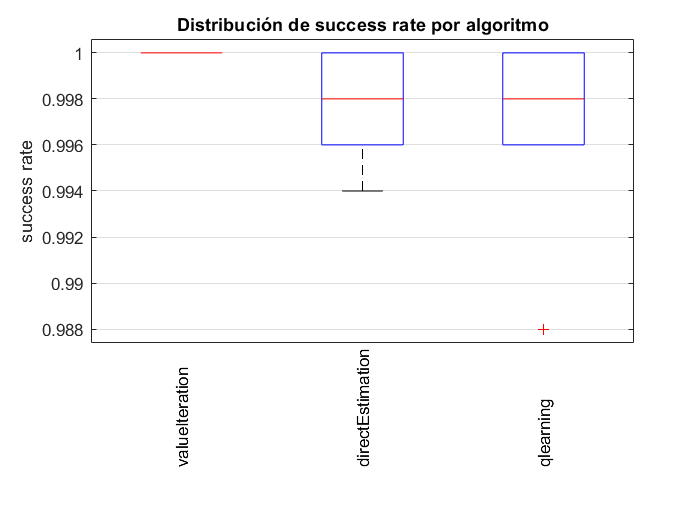
\includegraphics[width=0.8\textwidth]{../../experiments/algorithmsComparison/experiment/results/success.png}
    \caption{Tasa de éxito}
    \label{fig:algorithmsComparison-success}
\end{figure}

\begin{figure}[H]
    \centering
    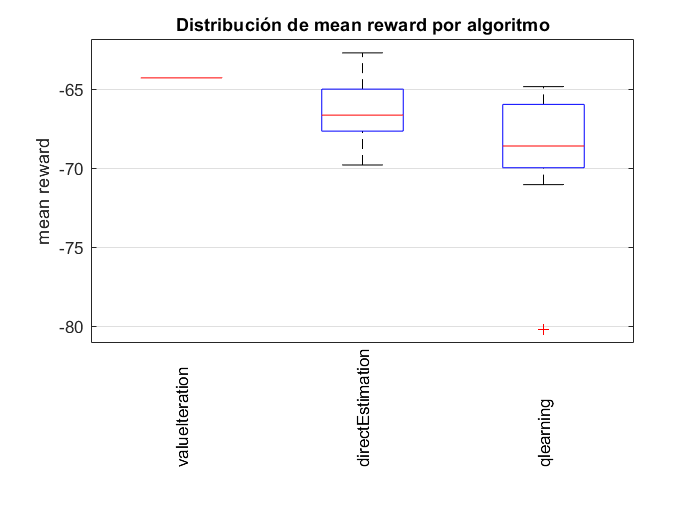
\includegraphics[width=0.8\textwidth]{../../experiments/algorithmsComparison/experiment/results/reward.png}
    \caption{Recompensa media}
    \label{fig:algorithmsComparison-reward}
\end{figure}

Se puede observar que \textit{Value Iteration} garantiza la política óptima una vez converge. Los otros dos métodos, \textit{Direct Estimation} y \textit{Q-learning}, tienen un pequeño sesgo y mayor varianza, reflejando la incertidumbre Monte Carlo y la exploración \epsilon-greedy.

\

Es interesante notar que \textit{Q-learning} es el algoritmo más rápido, a pesar de ser el que tiene mayor varianza. Sin embargo, su alta varianza puede llevar a resultados menos consistentes en comparación con \textit{Value Iteration} y \textit{Direct Estimation}, que son más estables pero más lentos.

\

El algoritmo \textit{Direct Estimation} es el más lento de los tres y tampoco produce una mayor recompensa media que el \textit{Value Iteration}, por lo que no es recomendable para este entorno.

\

Por consecuente, si se busca una solución rápida y eficiente, \textit{Q-learning} es la mejor opción. Sin embargo, si se busca una solución óptima y estable, \textit{Value Iteration} es el candidato más adecuado.